\documentclass[tikz,border=10pt]{standalone}
\usepackage{amsmath,amssymb}
\usepackage{tikz}
\usetikzlibrary{arrows,automata,backgrounds,calendar,chains,decorations,decorations.pathreplacing,decorations.text,fit,matrix,mindmap,patterns,petri,plotmarks,positioning,shadows,shapes,shapes.callouts,shapes.geometric,shapes.misc,spy,trees,calc,intersections,tikzmark,arrows.meta}
\usepackage{xcolor}
\usepackage{pgfplots}
\pgfplotsset{compat=1.16}

% Common math macros from the book
\def\x{\mathbf{x}}
\def\y{\mathbf{y}}
\def\z{\mathbf{z}}
\def\A{\mathbf{A}}
\def\b{\mathbf{b}}
\def\c{\mathbf{c}}
\def\w{\mathbf{w}}
\def\v{\mathbf{v}}
\def\u{\mathbf{u}}
\def\e{\mathbf{e}}
\def\zero{\mathbf{0}}
\def\R{\mathbb{R}}
\def\N{\mathbb{N}}
\def\Z{\mathbb{Z}}
\def\Q{\mathbb{Q}}
\def\st{\text{s.t.}}
\def\vect#1{\mathbf{#1}}
\def\xLP{x^{\mathrm{LP}}}
\def\zLP{z^{\mathrm{LP}}}
\def\xIP{x^{\mathrm{IP}}}

% Common node styles from the book
\tikzset{
    main/.style={circle, draw, fill=gray!20, minimum size=1cm, font=\normalsize},
    dot/.style={circle,fill=blue,minimum size=3pt,inner sep=0pt, outer sep=-1pt},
    vertex/.style={circle,fill=black!25,minimum size=20pt,inner sep=0pt},
    edge/.style={draw,-,thick},
    directed edge/.style={draw,->,>=latex,thick},
}

% Additional macros for 3D/coordinate systems
\newcommand{\xhat}{\hat{\x}}
\newcommand{\yhat}{\hat{\y}}
\newcommand{\zhat}{\hat{\z}}
\newcommand{\ihat}{\hat{\imath}}
\newcommand{\jhat}{\hat{\jmath}}
\newcommand{\khat}{\hat{k}}

\begin{document}
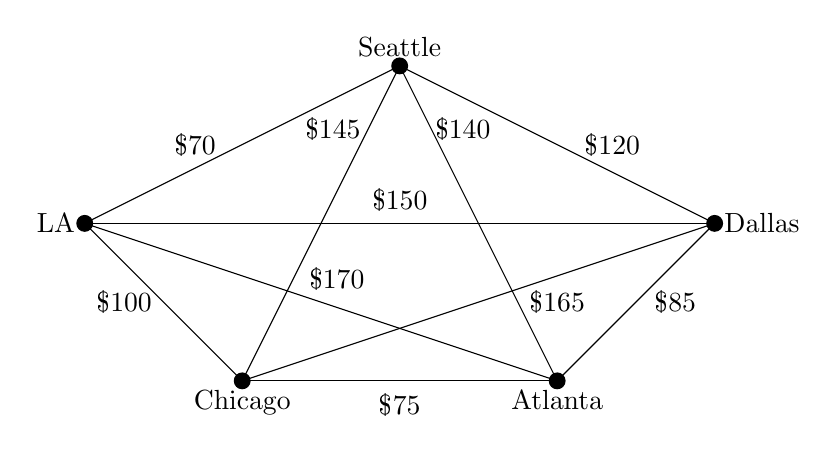
\begin{tikzpicture}
 \draw[fill] (0,0) circle[radius=.1] node[left]{LA};
\draw[fill] (2,-2) circle[radius=.1] node[below]{Chicago};
\draw[fill] (4,2) circle[radius=.1] node[above]{Seattle};
\draw[fill] (6,-2) circle[radius=.1] node[below]{Atlanta};
\draw[fill] (8,0) circle[radius=.1] node[right]{Dallas};
\draw(0,0)--(2,-2);
\node at (0.5,-1){\$100};
\draw(0,0)--(4,2);
\node at (1.4,1){\$70};
\draw(0,0)--(8,0);
\node at (4,0.3){\$150};
\draw(0,0)--(6,-2);
\node at (3.2,-0.7){\$170};
\draw(2,-2)--(4,2);
\node at (3.15,1.2){\$145};
\draw(4,2)--(6,-2);
\node at (4.8, 1.2){\$140};
\draw(4,2)--(8,0);
\node at (6.7,1){\$120};
\draw(2,-2)--(8,0);
\node at (6,-1){\$165};
\draw(2,-2)--(6,-2);
\node at (4,-2.3){\$75};
\draw(6,-2)--(8,0);
\node at (7.5,-1){\$85};
 \end{tikzpicture}
\end{document}
